\section{Early trips from the logbook}

\subsection{22.07.08 - Maillons and ladders in \protect\passage{M2}}

 \margininbox{M2}{
     \begin{itemize}
    \item Dan Greenwald
    \item Clewin Griffiths
    \end{itemize}}{\explo}

\begin{marginfigure}
\checkoddpage \ifoddpage \forcerectofloat \else \forceversofloat \fi
\centering
 \frame{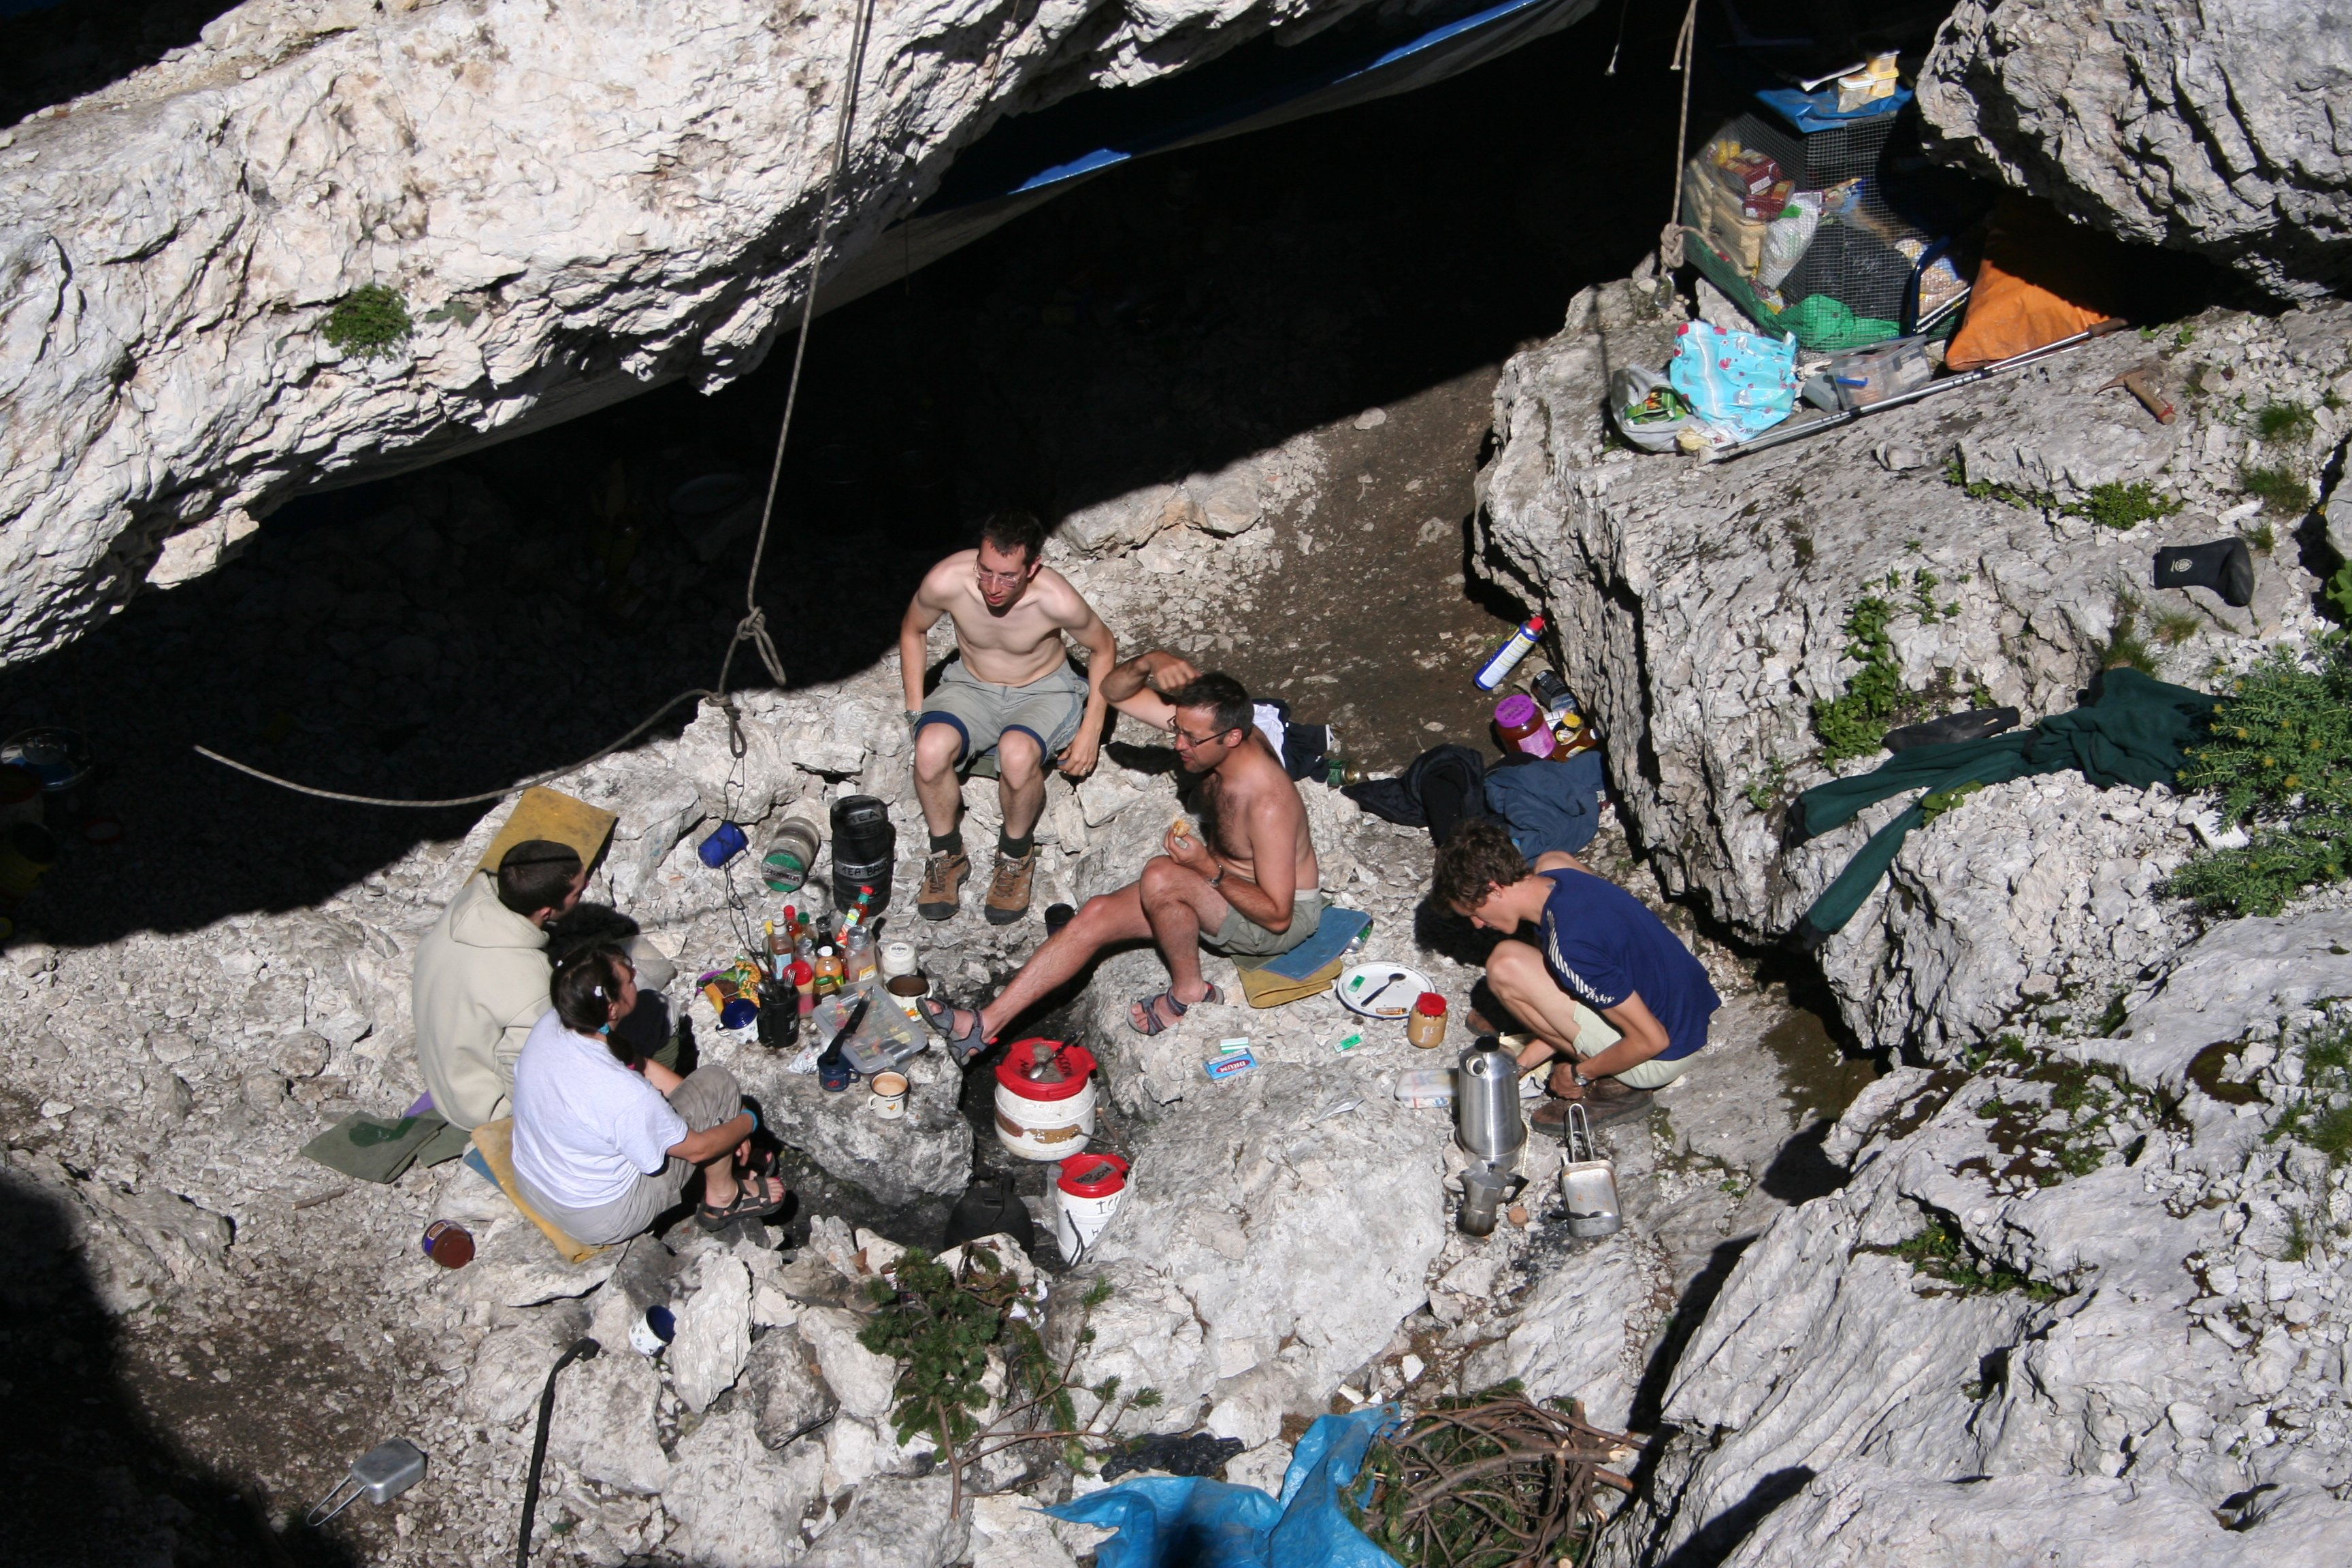
\includegraphics[width=\linewidth]{2008/logbook/Jana Carga - Canon 350D - img_3000 bivi on a sunny late morning--orig.jpg}} 
 \caption{The obligatory morning faff in the bivi takes just as long regardless of weather. \pic{Jana Čarga}}
 \label{sunny morning bivi}
\end{marginfigure}


\bignote{After the obligatory morning faff in the bivvy we started off for
\passage{M2}, then turned back after 20 metres} to get spits and cones.
Wandered over to the entrance which is a stone's throw from \passage{M18}.
The lower entrance drops into a gorgeous daylight shaft with a snow plug
in the bottom and vast amounts of scree.

We then followed the obvious way on, which rapidly gets less and less
obvious, turning into awkward rift. There are a fair few bits of free
climbing before we spotted a piton. Not wanting put all our trust into a
30 year old rusting bit of metal, we put in a couple of dodgy bolts as
back-ups to the piton. It was a straight drop, so we just used a few
metres of rope instead of one of the ladders we had. At the bottom is
ever squeezy and awkward rift ending in a ladder drop (another new
bolt). While doing this, Andy and James appeared, begging for maillons.
We had far too many anyway, so we sent them off happy. At the end of the
ladder drop awaited yet more rift and free climbs. The last climb we
rigged with ladder before taking it off again since it didn't seem to
buy us anything. There it opened out into a reasonable, i.e.~more than 2
m, pitch. We put in two more bolts and then ran into trouble on the
third. Dan bludgeoned the spit teeth into a pulp and we spent about 10
minutes trying ingenious ways to remove the duff spit from the driver.
But we didn't want to do anything which would make it too difficult to
remove if things went wrong. It was already 7:30 pm so we abandoned the
mission.

\name{Clewin Griffiths}

\subsection{22.07.08 - Rerigging \protect\passage{Laurel}}

 \margininbox{Vrtnarija}{
     \begin{itemize}
    \item Andrew Jurd
    \item James Kirkpatrick
    \end{itemize}}{\explo}

Set off at 1-ish to rerig \passage{Laurel}. Got to the
top of \passage{Laurel} and found the ropes, but not maillons! Decided to
walk back to bivvy and look for more. Having found none, we left for
\passage{M2} to look for Clew and Dan and their stash of maillons. After a
LONG search for \passage{M2}, we reach \passage{M2} and start going through loose meanders, constantly worried that we were going to shower Dan and Clew in
rock fall. Eventually we get the maillons, walked back to GW, finally
rig \passage{Laurel}. The second rope on \passage{Laurel} is slightly worn and
could do with changing (15-20 m rope needed).

\name{James Kirkpatrick}

\subsection{Captain Kangaroo}

\margininbox{Captain Kangaroo}{
    \begin{itemize}
    \item Jana Čarga
    \item James "Tetley" Hooper
    \item James Huggett
    \end{itemize}}{\explo}

Easy down to \passage{Laurel}. First rebelay under the boulder turned out
to be too tight for our shorter members: add a long sling.

Down to \passage{Pico} no problem, then to \passage{Bonus Chamber},
\passage{Scrotty} would do with some mechanical enlarging. Down to
\passage{Traverse Chamber}. Left 20 m of rope, 5x spit, maillon, hangers,
cones. Rigged a free climb to \passage{Mudslump} (could be improved).

\name{Tetley}

First trip for me down to \passage{Mud Slump}. Lovely trip. It is
actually not that scrotty - at least, not for me\ldots{} :) \passage{Pico}
is an amazing pitch. Will definitely return down there!

\name{Jana Čarga}

   \margininbox{Name translations}{
     \begin{itemize}
    \item Captain Kangaroo – Kapitan Kenguru
    \item Bonus Chamber – Dvorana bonus
    \item Mud Slump – Blatni sifon (Mud sniffles / siphon)
    \item Olympic Rift – Olimpijski meander
    \item Traverse Chamber – Dvorana traverza
    \end{itemize}}{\logbook}

\subsection{\protect\passage{M2} Rigging Part 2}

 \margininbox{M2}{
     \begin{itemize}
    \item Dan Greenwald
    \item Clewin Griffiths
    \end{itemize}}{\explo}
 

Started where we left off --- with 2 ½ bolts placed at
the top of the first real pitch. Dan finished off the last bolt and so
we abseiled down. Using the rope from the pitch I climbed up from the
bottom to see if there was a way on at a high level. There wasn't, but
\bignote{the aven looks promising, although would require a proper climbing trip}.
The bottom of the pitch leads to a 40 m pitch. There was a 70s piton for
backup and a spit at the pitch head. We used the spit (not \textit{too}
rusty) and put a new spit to give a Y-hang. 30 m down was a wide ledge
with garbage from the 70s.

Side track: Off the ledge was a small rift leading to a drop which
we rigged with a ladder. Below that a dodgy free climb lead to a nice
section of wide rift passage with a stream at the bottom and a red
survey dot on the wall. This all closed up completely, so we derigged
the ladder.

At the bottom of the 40 m (\passage{Kletnikov Skropilnik}) a tight rift of black
rock lead to the next pitch. There were no pitch head bolts so we left
this for another trip. 

\name{Clewin Griffiths}

\subsection{25.07.08 - Investigating possibilities in E1\ldots{}}

 \margininbox{E1}{
     \begin{itemize}
    \item Jana Čarga
    \item Jarvist Frost
    \end{itemize}}{\explo}

\begin{marginfigure}
\checkoddpage \ifoddpage \forcerectofloat \else \forceversofloat \fi
\centering
 \frame{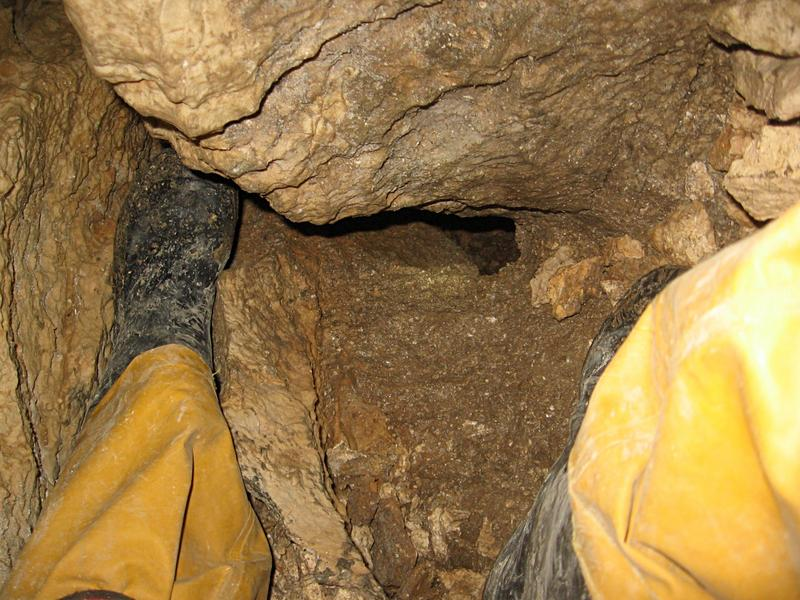
\includegraphics[width=\linewidth]{2008/logbook/Jarvist Frost - canon a520 - e1 - new pitch head.jpg}} 
 \caption{The new pitch head in E1. \pic{Jarvist Frost}}
 \label{pitch head e1}
\end{marginfigure}

Jana pushed the small crawl, which was draughting; went for a while.

We then moved attention to the deep deep crawl, abandoned last year as
dead. It wasn't. But perhaps it should have been. We moved the most
dangerous boulder loitering over the edge and set to work.

Dig dig dig\ldots{}

6 m long, $\approx$ 60° scree slope, terminating in pitch (6-8 m,
as judged by rattling stones).

First few armfuls of rock were stacked, until we started chucking scree
over the edge, boom boom boom. Tidied back to bedrock - too tight -
damn! Strange pitch head, almost T-shaped: water slopping over the edge,
but also a notch cut down ($\approx$ 10 cm wide).

We surface surveyed and tied the centreline to \passage{M2} entrance.
The end of the cave is 40 m above the end of \passage{Goodybag}, \passage{M16}.

We will need a better name before it gets too big → `Mountain Goat
Cave'? Sounds good in Slovene, says Jana.

\name{Jarvist Frost}


\subsection{26.07.08 - 3rd rig of \protect\passage{M2}}

 \margininbox{M2}{
     \begin{itemize}
    \item Andrej Fratnik
    \item James Kirkpatrick
    \end{itemize}}{\explo}

Continued where we left: Andrej rigged \passage{M2}: safely 1st rebelay on
a giant (minibus sized) boulder of dubious stability. 2hrs + 5 rebelays
later we were 20 m from the bottom and out of spits. Damn! Return with 5+
bolts and finish the job some other day. Had a hell of a time getting
out of the entrance rift\ldots{}

\name{James Kirkpatrick}









\subsection{26.07.08 - \passage{M16} $\rightarrow$ \passage{Plopzilla} $\rightarrow$ end of \passage{NCB} (\passage{Zebra} passage)}

 \margininbox{M16}{
     \begin{itemize}
    \item Jana Čarga
    \item Andrew Jurd
    \end{itemize}}{\explo}

10 hour trip. 
Re-rigged the way down to \passage{Gladiators'}. 

Also re-rigged a small traverse just after \passage{Club Mig}.

Jana had an epic piss on the ledge in the middle of \passage{Gladiators' Traverse.} 

\margininbox{For Evans' Sake, 2009}{
     "Jana Čarga for her mid Gladiator's traverse relieving of bladder pressure, perched above twin 60m pitches on a wedged rock, with one leg through a harness loop for 'safety'."}{\award}

We check out \passage{Plopzilla}, but have not taken the rope out.

Checked the end of \passage{NCB}. In \passage{Zebra}, 2 ways on:

\begin{enumerate}
    \item 
    A small climb down ($\approx$ 6 m) need to be smashed, remove boulders
    \item 
    Small, tight crawl continuing up \passage{Zebra}
\end{enumerate}

Have taken the Gladiator's old rope out. Amazing trip!
    
\name{Jana Čarga}




\begin{figure*}[b]
\checkoddpage \ifoddpage \forcerectofloat \else \forceversofloat \fi
\centering
    \begin{subfigure}[b]{0.49\textwidth}
        \centering
        \frame{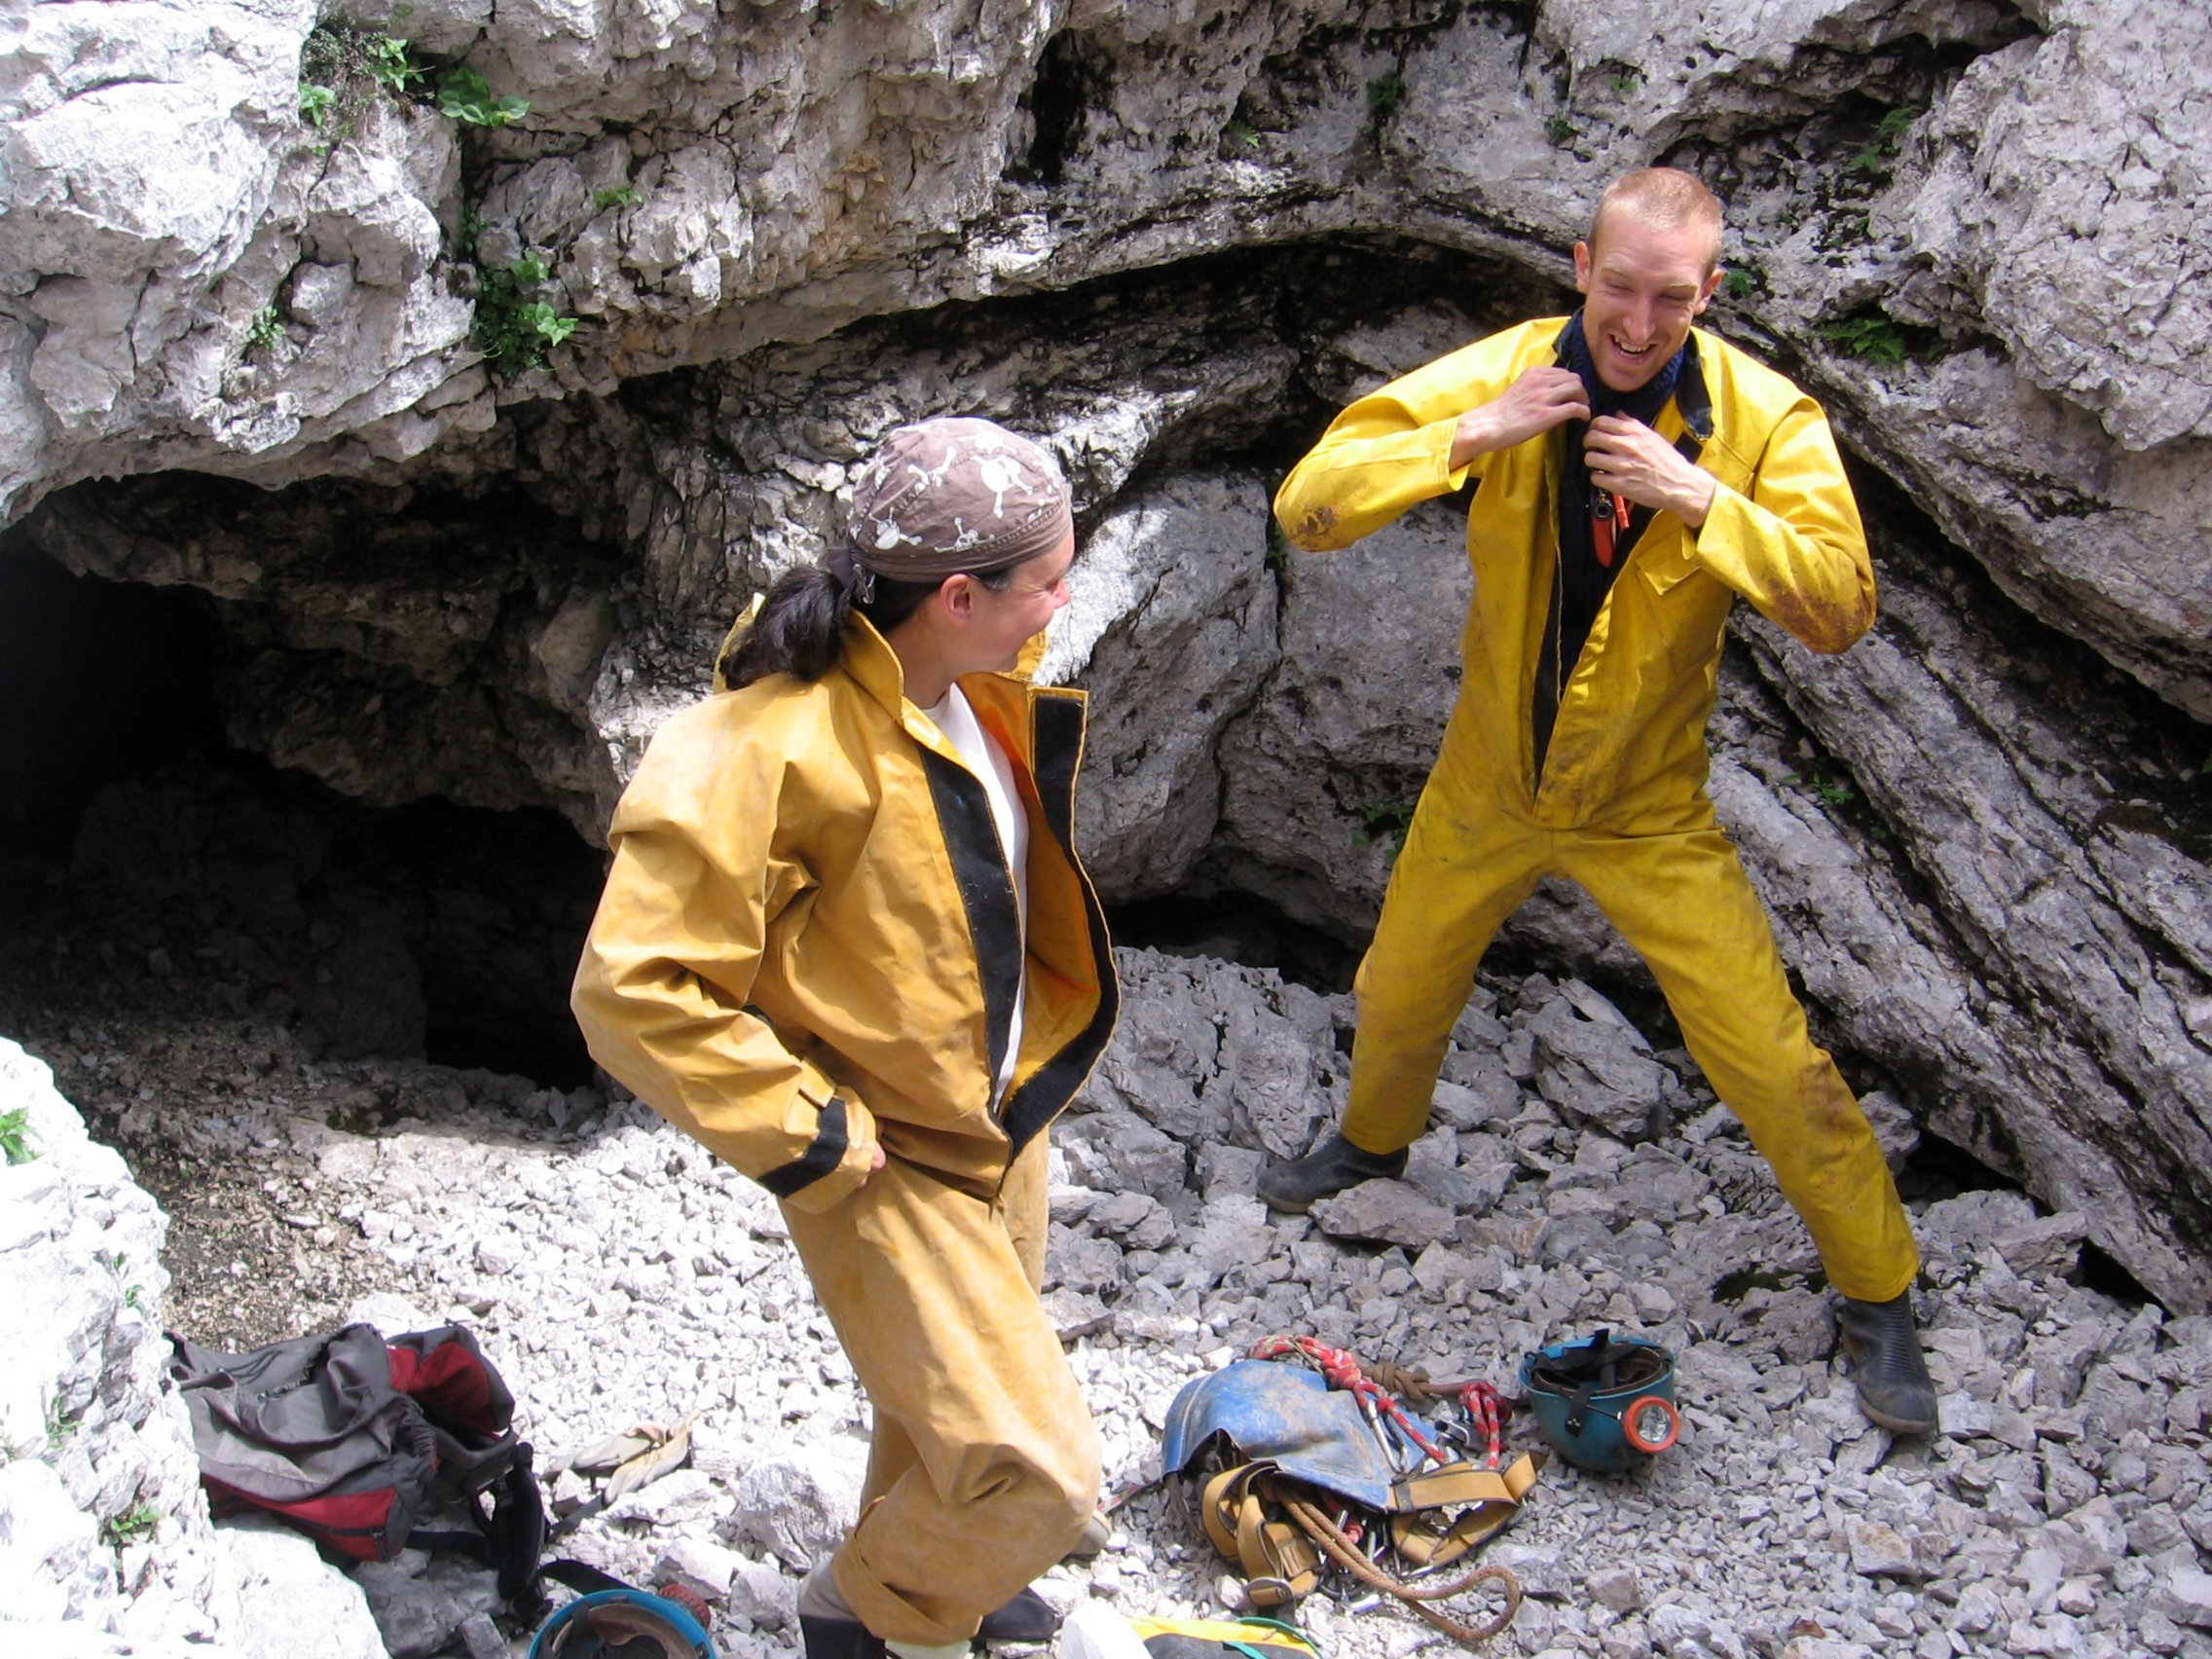
\includegraphics[width=\linewidth]{2008/logbook/Jarvist Frost - canon a520 - sysmig - JC AJ trip - getting ready--orig.jpg}} 
        \caption{} \label{M16 prep}
    \end{subfigure}
        \hfill
\begin{subfigure}{0.49\textwidth}
\centering
\frame{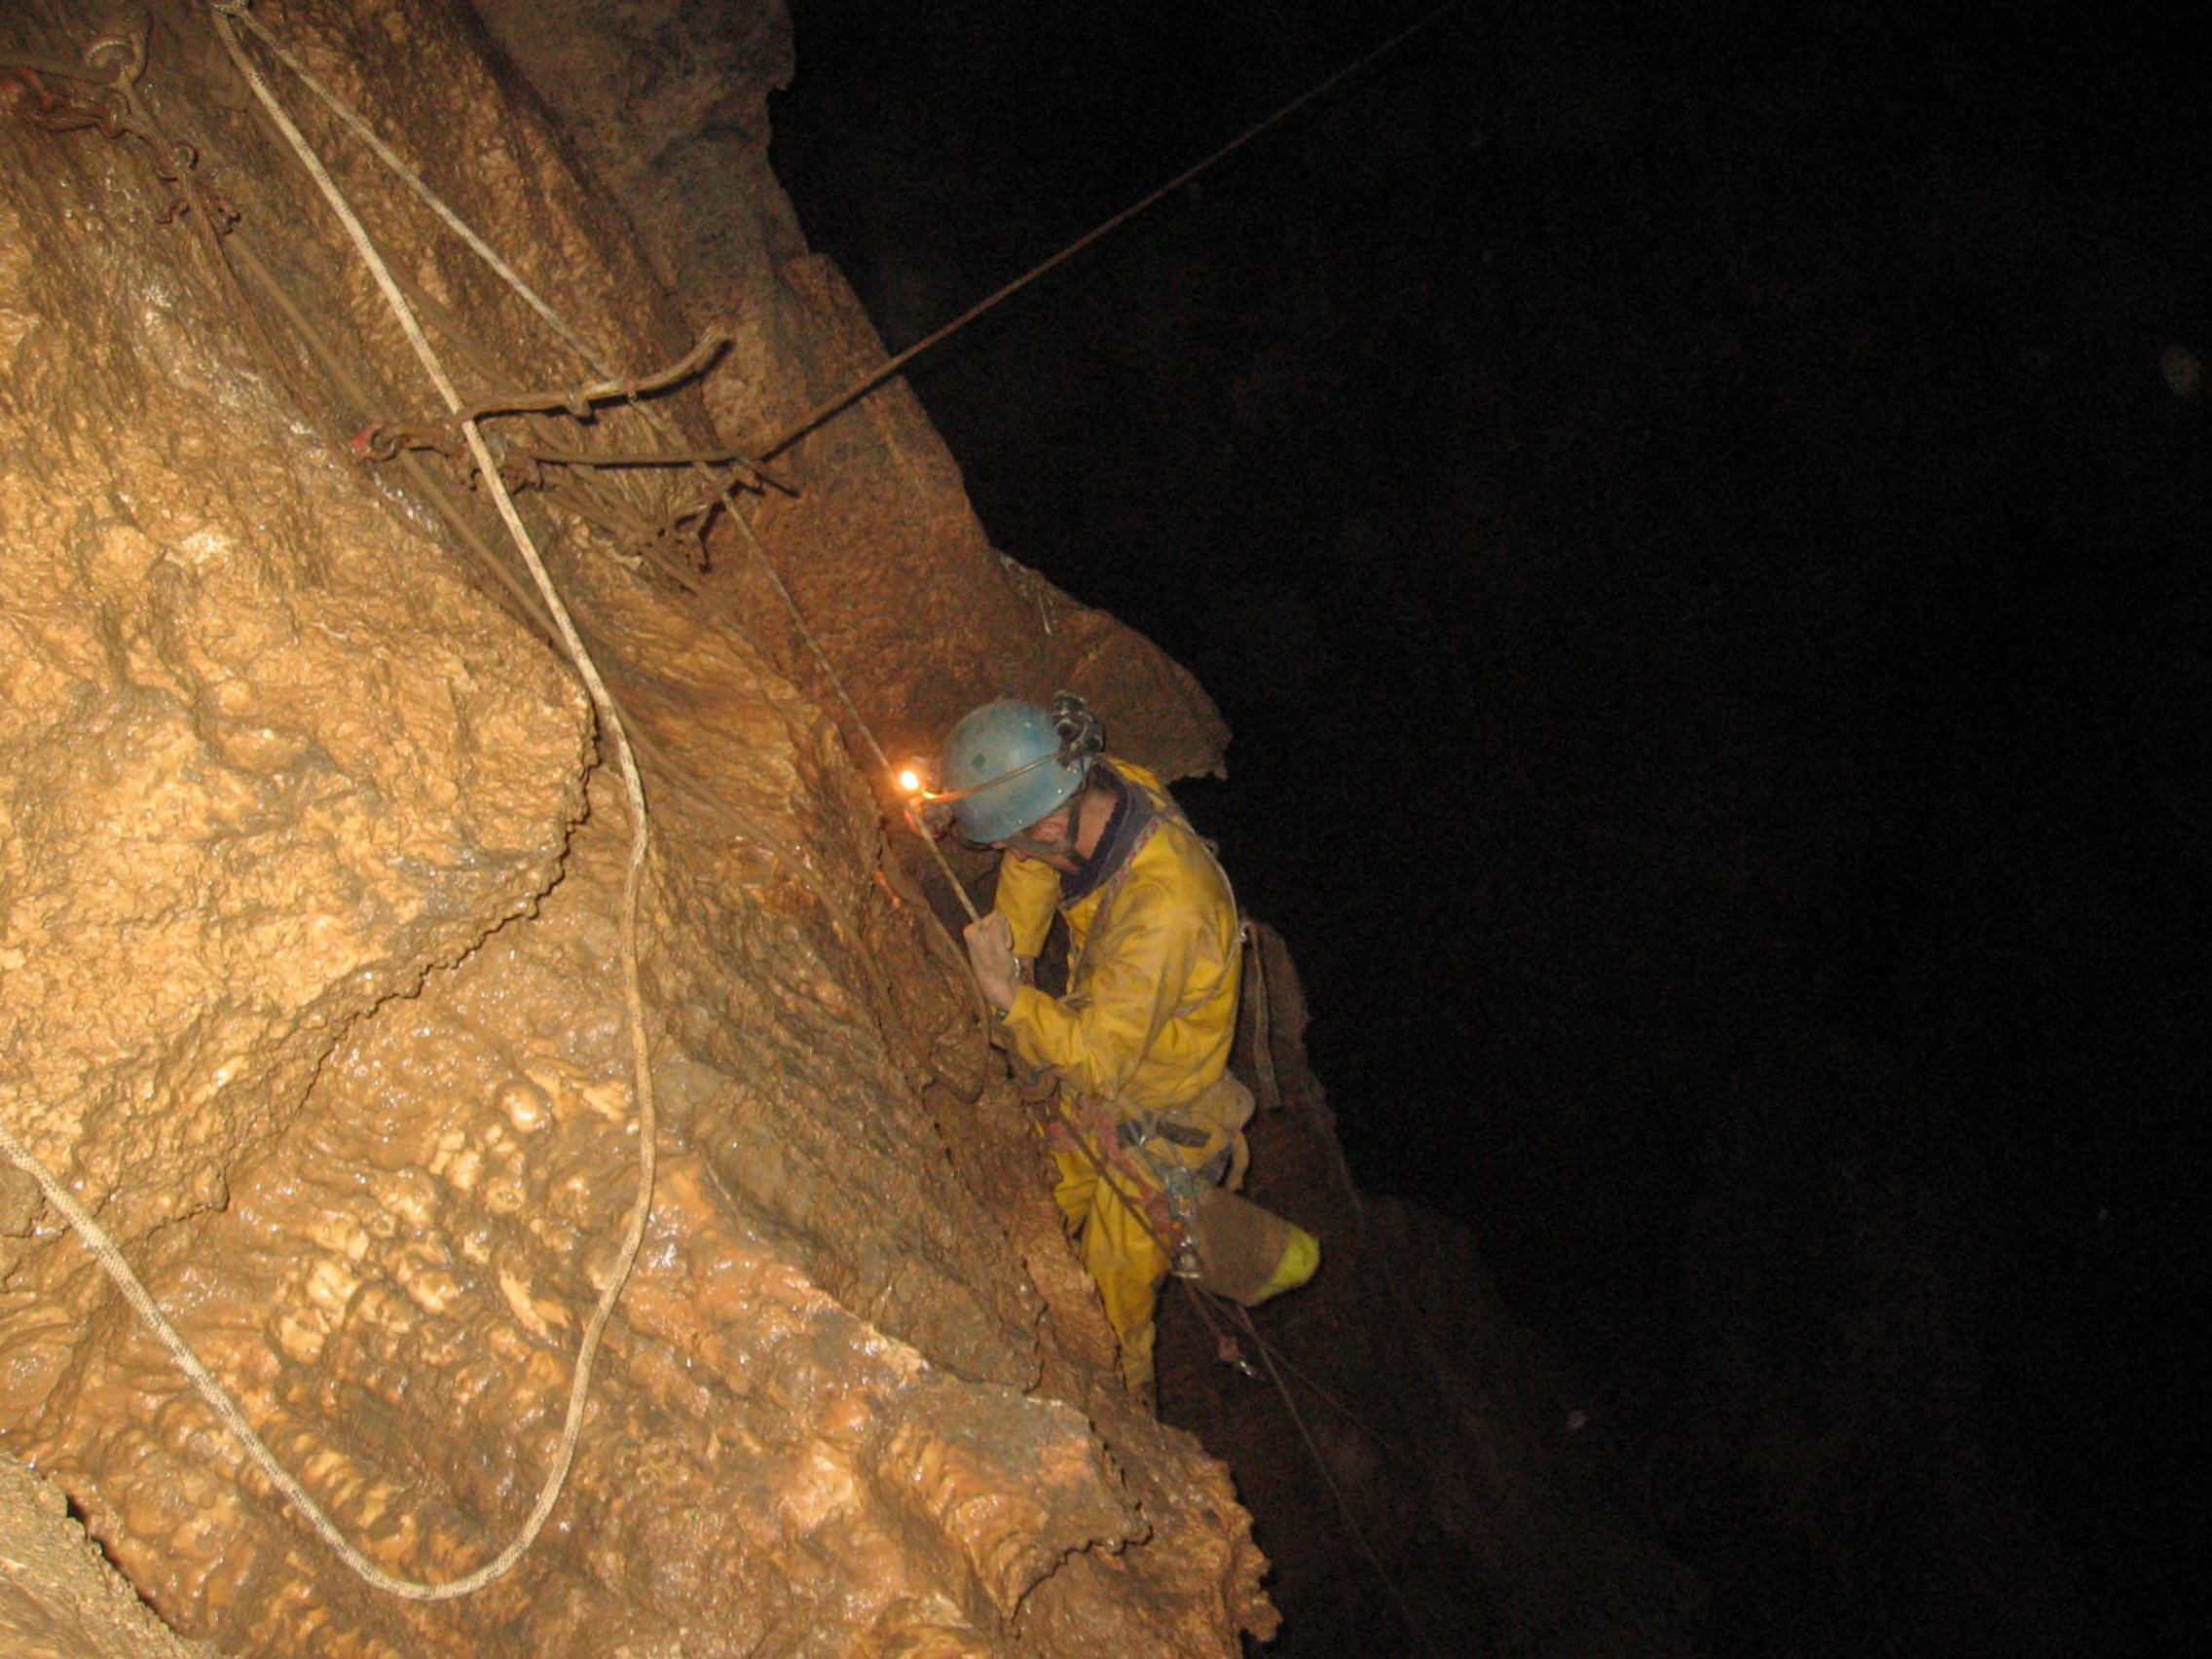
\includegraphics[width=\linewidth]{2008/logbook/Jarvist Frost - canon a520 - sysmig - JC AJ trip - Andy on gladiators--orig.jpg}}
 \caption{}\label{gladiators}
\end{subfigure}
  \caption{A trip into \passage{M16}. \textit{(a)} Andy and Jana kitting up for the trip outside \passage{M16}. \pic {Jarvist Frost} \textit{(b)}Andy negotiating the \passage{Gladiator's traverse}. \pic {Jana Čarga}}
\end{figure*}


